\documentclass[11pt,a4paper]{article}
\usepackage[T1]{fontenc}
\usepackage{lmodern}
\usepackage[margin=2.5cm]{geometry}
\usepackage{amsmath,amssymb}
\usepackage{booktabs}
\usepackage{array}
\usepackage{enumitem}
\usepackage{xcolor}
\usepackage{graphicx}
\graphicspath{{figures/residual/}}
\PassOptionsToPackage{hyphens}{url}
\usepackage[colorlinks=true,linkcolor=blue!50!black,urlcolor=blue!50!black]{hyperref}

\renewcommand{\Re}{\operatorname{Re}}
\renewcommand{\Im}{\operatorname{Im}}
\newcommand{\dext}{\delta_{\rm ext}}
\newcommand{\Lop}{\mathcal{L}_\ell}
\newcommand{\x}{\mathbf{x}}
\newcommand{\code}[1]{\texttt{#1}}
\newcommand{\psiR}{\tilde\psi^{\rm R}_\ell}
\newcommand{\phiR}{\phi^{\rm R}_\ell}

\title{Extracting the second-order residual field at the particle\\[4pt]
\large A toy-model test of Taylor continuation from the contour}
\author{Draft prepared with Claude Code for Andrew Spiers (UCD)}
\date{16 October 2026}

\begin{document}
\maketitle

\begin{abstract}
The contour method gives the second-order field on a complex contour inside the worldtube and on the real line outside it.
That is enough for fluxes, but a local self-force also needs the second-order residual field, and its gradient, at the particle.
We test whether this can be obtained by subtracting a continued second-order puncture from the contour solution, where both are of order one, and continuing the difference analytically from the contour to $r_0$ by a Taylor series generated from the radial ODE.
In the flat-space toy model with $Q=\tfrac12\partial_Z^2(AB)$ and the exact second-order singular field, the continued residual is analytic at $r_0$.
The Taylor series converges geometrically, with the ratio set by the distance to the next singularity at $z=0$, and recovers every residual mode and its radial derivative at $r_0$ to $10^{-32}$.
The mode sums for $\Phi_2^{\rm R}(\x_0)$ and $\partial_r\Phi_2^{\rm R}(\x_0)$ are then limited only by $\ell$-truncation.
With deliberately truncated punctures the continued residual has a branch point at $r_0$, and convergence becomes algebraic: $N^{-(k+2)}$ for a puncture error $\propto\rho^k$, two orders better than the 3D smoothness suggests.
A simpler baseline, reading the residual at $r_0+i\eta$ on lower contours and extrapolating $\eta\to0$, also works, without the cancellation we had expected.
The toy is static, so it tests the extraction of the local residual but not the split into dissipative and conservative parts.
\end{abstract}

{\small\tableofcontents}

\section{Question and summary}
The contour method solves for the full second-order field.
Inside the worldtube the modes are known on the contour $z=y(a)$; outside, on the real line.
The fluxes at the boundaries follow directly.
A local self-force needs more: the regular (residual) part of the field and its gradient at the particle, $\Phi_2^{\rm R}(\x_0)$ and $\nabla\Phi_2^{\rm R}(\x_0)$.
In mode language, these are the residual modes $\phiR(r_0)$ and $\partial_r\phiR(r_0)$, summed over $\ell$.

The proposal tested here has two steps.
\begin{enumerate}[leftmargin=*]
\item On the contour, subtract the continued second-order puncture from the contour solution, $\psiR(z)=\tilde\psi_\ell(z)-\tilde\phi^{\rm P}_\ell(z)$.
On the contour $|z-r_0|\ge0.298$, so both terms are of order one and no singular quantity is subtracted from another.
\item Continue $\psiR$ from the contour to $r_0$ with a Taylor series, and take its real part.
\end{enumerate}

\paragraph{Summary of results.}
\begin{itemize}[leftmargin=*]
\item \emph{Exact puncture:} the continued residual is analytic at $r_0$ (its monodromy around $r_0$ is below $4\times10^{-20}$).
The Taylor series about the apex $r_0+i$ converges geometrically with ratio $0.199$, against the predicted $|r_0-z_e|/|z_e|=0.196$.
It recovers $\phiR(r_0)$ and $\partial_r\phiR(r_0)$ for all $\ell\le20$ to better than $10^{-34}$ and $10^{-32}$, reaching $10^{-20}$ after 29--50 terms.
\item \emph{Mode sums:} $\Phi_2^{\rm R}(\x_0)$ and $\partial_r\Phi_2^{\rm R}(\x_0)$ have errors $9.6\times10^{-11}$ and $4.1\times10^{-10}$ at $\ell_{\max}=20$, entirely from $\ell$-truncation.
\item \emph{Truncated punctures} $\Phi_2^{\rm P}=\Phi_2^{\rm S}+\epsilon q^2\rho^k$: the convergence is algebraic, with value errors $\propto N^{-(k+2)}$ (fitted slopes $-3.0$, $-5.1$, $-7.3$ for $k=1,3,5$).
\item \emph{Baseline:} reading the residual at $r_0+i\eta$ has a bias $-\eta\,\Im\psiR{}'(r_0)$; Richardson extrapolation over $\eta=1,\dots,1/128$ recovers the exact case to $3\times10^{-15}$--$5\times10^{-11}$.
\item \emph{Controls:} continuing the puncture one-sidedly (dropping its kink at $r_0$) fails, as it should.
Blending the finished, kinked puncture modes with $H$ works, contrary to our prediction (Sec.~\ref{sec:controls}).
\end{itemize}

\section{Set-up}\label{sec:setup}

\subsection{Toy model and contour}
The first-order field satisfies $\nabla^2\Phi_1=-4\pi q\,\delta^3(\x-\x_0)$, with
\begin{equation}
\Phi_1=\frac q\rho+\Phi^{\rm R}_1,\qquad \Phi^{\rm R}_1=c_0+c_1Z=A+c_1d,\qquad A=c_0+c_1r_0,
\end{equation}
where $Z=r\mu$ is the Cartesian coordinate along the axis, $\x_0=r_0\hat Z$, and $d=Z-r_0$.
The second-order field satisfies $\nabla^2\Phi_2=\tfrac12\partial_Z^2(\Phi_1^2)$.
Its exact solution is $\Phi_2=\tfrac12\partial_Z^2\chi$, with $\nabla^2\chi=\Phi_1^2$.
The parameters are $q=1$, $r_0=5$, $c_0=1$, $c_1=1/10$, on the domain $r\in[1,10]$.
The contour is $y(a)=a+i\big(1-4(a-r_0)^2\big)^6$ on $[a_L,a_R]=[4.5,5.5]$, with apex $r_0+i$.
The radial operator is $\Lop\psi=\psi''+2\psi'/r-\ell(\ell+1)\psi/r^2$.

\subsection{The exact second-order singular field}
Write $\Phi_1^2=q^2/\rho^2+2qA/\rho+2qc_1d/\rho+(\Phi_1^{\rm R})^2$.
Using $\nabla^2\ln\rho=1/\rho^2$, $\nabla^2\rho=2/\rho$ and $\nabla^2(d\rho)=4d/\rho$, the singular part of $\chi$ is
\begin{equation}
\chi^{\rm S}=q^2\ln\rho+qA\rho+\tfrac12qc_1\,d\rho,\qquad
\Phi_2^{\rm S}=\tfrac12\partial_Z^2\chi^{\rm S},
\label{eq:PhiS}
\end{equation}
with the derivative taken in the distributional sense.
Then $\Phi_2^{\rm R}=\Phi_2-\Phi_2^{\rm S}=\tfrac12\partial_Z^2(\chi-\chi^{\rm S})$ is smooth at $\x_0$.
Because $\Phi_1^{\rm R}$ is linear, the singular field is a finite closed form.
In GR, and in any toy with a non-polynomial regular field, it is an infinite local series that must be truncated.

\subsection{An injected regular field}
With the boundary data used in earlier stages, the SS and SR solutions equal $\tfrac12\partial_Z^2$ of the singular parts of $\chi$ exactly.
The residual from SS and SR would then vanish identically, and the test would be trivial.
To give every $\ell$ a nonzero residual, the agent added a harmonic field through the Cauchy data at $a_L$:
\begin{equation}
h=\frac{B_o}{|\x-r_o\hat Z|}+\frac{B_i}{|\x-r_i\hat Z|},\qquad B_o=10,\ r_o=15,\ B_i=1,\ r_i=\tfrac12,
\end{equation}
which is harmonic on the domain.
Its modes are $h_\ell(r)=\sqrt{4\pi/(2\ell+1)}\,\big[B_o r^\ell/r_o^{\ell+1}+B_i r_i^\ell/r^{\ell+1}\big]$.
The RR piece is solved on the real line, as before, and is regular at $r_0$.
The exact residual values at the particle are
\begin{align}
\Phi_2^{\rm R}(\x_0)&=\tfrac16c_0^2+\tfrac35c_0c_1r_0+\tfrac12c_1^2r_0^2+h(\x_0)=1.81388888888888888889,\\
\partial_r\Phi_2^{\rm R}(\x_0)&=0.16061728395061728395.
\end{align}
On the axis $\partial_r=\partial_Z$, and by axisymmetry this is the whole gradient.

\section{Method}\label{sec:method}

\subsection{The contour solution and the continued puncture}
SS and SR are solved together on the contour by variation of parameters, with 60 Gauss panels of 20 nodes in $a$ and closed-form sources evaluated at 50 digits.
This agrees with the NDSolve contour solve of the earlier stages to $10^{-15}$.
The continued sources are those of Stage~9: $\tilde s_{\rm SS}$ with $2\log(z+r_0)-2\log(z-r_0)$, and $\tilde s_{\rm SR}$ through the $\Theta\to H$ continuation of the coupling kernels.

The continued puncture $\tilde\phi^{\rm S}_\ell$ is built in the same way as the source:
\begin{itemize}[leftmargin=*]
\item \emph{SS part:} the modes of $\tfrac12\partial_Z^2(q^2\ln\rho)$ are the same real function on both sides of $r_0$, with $\ln|r-r_0|$.
They are continued by $\ln|r-r_0|\to\log(z-r_0)$.
\item \emph{SR part:} the undifferentiated modes $F_j=[\chi_{\rm SR}]_j$ are $C^2$ at $r_0$.
They are continued by the blend $F_{\rm in}+(F_{\rm out}-F_{\rm in})H$, with $H=1+\tfrac{i}{\pi}\log(z-r_0)$, and then the $\tfrac12D_z^2$ ladder is applied.
\end{itemize}
Three identities were checked:
\begin{itemize}[leftmargin=*]
\item $\tilde s_{\rm SS}=\Lop\tilde\phi^{\rm S}_{\rm SS}$ exactly ($10^{-40}$);
\item $\Re\tilde\phi^{\rm S}_\ell(r+i0)$ equals the modes of $\Phi_2^{\rm S}$ on both sides of $r_0$;
\item the residual source $\tilde s^{\rm R}=\tilde s_{\rm SS}+\tilde s_{\rm SR}-\Lop\tilde\phi^{\rm S}_\ell$ is imaginary on the axis and bounded at $r_0$.
\end{itemize}
The last of these is expected: the physical residual source of SS and SR is zero, so only a shadow is left.

\subsection{Why the residual should be analytic at \texorpdfstring{$r_0$}{r0}}
$\psiR$ is analytic between the contour and the real axis.
Its real part on the axis is the physical residual mode, which for the exact puncture is real-analytic at $r_0$ and contains no $\delta$ terms.
Subtracting the analytic continuation of that real part leaves a function whose real part vanishes on the axis.
By Schwarz reflection, such a function extends analytically across the axis, including through $r_0$.
So $\psiR$ should be analytic in a disc around $r_0$, and a Taylor series about a contour point $z_e$ should converge at $r_0$ with ratio $|r_0-z_e|/|z_e|$, set by the regular singular point of $\Lop$ at $z=0$.

With a truncated puncture, the physical residual is only finitely differentiable at $r_0$.
Its continuation then contains a term like $(z-r_0)^m\log(z-r_0)$, so $r_0$ is a branch point on the edge of every Taylor disc and convergence can only be algebraic.

\subsection{Taylor coefficients from the ODE}
Fitting Taylor coefficients to values on the contour would be numerical continuation off a curve, which is exponentially ill-conditioned.
Instead the coefficients are generated by the ODE itself.
With $z=z_e+w$ and $\psiR=\sum_n p_nw^n$, the equation $z^2\psi''+2z\psi'-\ell(\ell+1)\psi=z^2\tilde s^{\rm R}$ gives
\begin{equation}
p_{n+2}=\frac{\sigma_n-2z_e(n+1)^2p_{n+1}-\big[n(n+1)-\ell(\ell+1)\big]p_n}{z_e^2(n+2)(n+1)},
\label{eq:recursion}
\end{equation}
where $\sigma_n$ are the Taylor coefficients of $z^2\tilde s^{\rm R}$ about $z_e$.
The starting values $p_0=\psiR(z_e)$ and $p_1=\psiR{}'(z_e)$ come from the contour solve.
The $\sigma_n$ come from a Cauchy integral of the source on the circle $|z-z_e|=0.7|z_e-r_0|$, using the trapezoidal rule with 256 points.
Every quantity involved is of order one.
The partial sums at $r_0$ are
\begin{equation}
S_N=\sum_{n\le N}p_n(r_0-z_e)^n,\qquad S'_N=\sum_{n\le N}n\,p_n(r_0-z_e)^{n-1}.
\end{equation}
Two expansion points were used: the apex $a_e=5$ ($|z_e-r_0|=1$) and $a_e=5.2$ ($|z_e-r_0|=0.404$).
As a cross-check, the residual ODE was also solved around a circle $|z-z_e|=r_c$ and the coefficients taken by Cauchy integrals.
These agree with the recursion to $2\times10^{-19}$ in the coefficients and $6\times10^{-16}$ in the partial sums at $N=40$.

\section{Results}\label{sec:results}

\subsection{The residual on the contour}
Figure~\ref{fig:contour} shows $\psiR$ along the contour for several $\ell$.
Its real part at $a_L$ and $a_R$ equals the physical residual there, as required.
Its imaginary part, the shadow, is of order one and grows with $\ell$: $\Im\psiR(a_R)$ reaches $-11$ at $\ell=20$.
Since $\phiR(r_0)=1.1\times10^{-10}$ at $\ell=20$, the extraction recovers a small real part beside a large imaginary one.
At the 50 digits used here this costs nothing, but in double precision the absolute accuracy of a high-$\ell$ mode would be set by the size of the shadow, not by the size of the residual.

\begin{figure}[t]
\centering
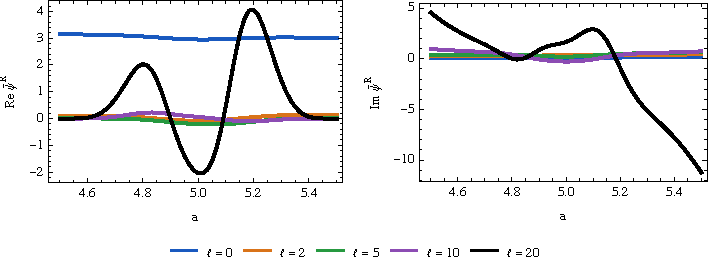
\includegraphics[width=0.9\textwidth]{fig_residual_contour.pdf}
\caption{The residual $\psiR=\tilde\psi_\ell-\tilde\phi^{\rm S}_\ell$ along the contour, exact puncture. Left: real part; right: imaginary part (the shadow).}
\label{fig:contour}
\end{figure}

\subsection{Exact puncture: geometric convergence}
Table~\ref{tab:exact} lists the extracted residual modes.
For every $\ell\le20$ the real part of the Taylor sum at $r_0$ equals the exact $h_\ell(r_0)$ to better than $10^{-34}$, and the radial derivative to better than $10^{-32}$, which is the floor of the 50-digit arithmetic.
A fit $|p_n(r_0-z_e)^n|\sim n^c\varrho^n$ to the coefficients gives $\varrho=0.199$ at the apex and $0.080$ at $a_e=5.2$, against the predicted $0.196$ and $0.078$.
The monodromy of $\psiR$ around $r_0$ is below $4\times10^{-20}$, so $r_0$ is not a singular point.
Every contour point works, and points closer to $r_0$ converge faster.

The value $\Im\psiR(r_0)$ is of order one: the shadow is carried to $r_0$, but only the real part is physical.

\begin{table}[t]
\centering
\caption{Exact puncture: residual modes at $r_0$ from the Taylor series about the apex ($N=120$). $N_{20}$ is the number of terms needed for $10^{-20}$.}
\label{tab:exact}
\begin{tabular}{rllllr}
\toprule
$\ell$ & $\Re S_N=h_\ell(r_0)$ & value error & derivative error & $\Im\psiR(r_0)$ & $N_{20}$\\
\midrule
0 & $3.0722533415696$ & $<10^{-36}$ & $<10^{-34}$ & $0.144$ & 29\\
2 & $0.12060258176715$ & $<10^{-36}$ & $<10^{-34}$ & $0.320$ & 32\\
5 & $2.9344555955148\times10^{-3}$ & $<10^{-35}$ & $<10^{-33}$ & $0.455$ & 34\\
10 & $8.7335788933812\times10^{-6}$ & $<10^{-35}$ & $<10^{-32}$ & $0.505$ & 39\\
15 & $2.9581078715916\times10^{-8}$ & $<10^{-34}$ & $<10^{-32}$ & $0.184$ & 46\\
20 & $1.0585141067450\times10^{-10}$ & $<10^{-34}$ & $<10^{-32}$ & $-1.171$ & 50\\
\bottomrule
\end{tabular}
\end{table}

\subsection{Truncated punctures: algebraic convergence}
To mimic GR, where punctures are always truncated, the puncture was replaced by $\Phi_2^{\rm P}=\Phi_2^{\rm S}+\epsilon q^2\rho^k$ with odd $k=1,3,5$ and $\epsilon=r_0^{-(k+2)}$.
The 3D residual is then $C^{k-1}$, and its exact value at $\x_0$ is unchanged because $\rho^k$ vanishes there.
This is the second-order analogue of the $cq\rho^n$ trick used for first-order punctures in Stage~6.

Figure~\ref{fig:taylor} and Table~\ref{tab:rates} show the result.
Convergence is algebraic, as predicted, but with the exponent $k+2$, not $k$:
\begin{itemize}[leftmargin=*]
\item The mode functions $[\rho^k]_\ell$ are $C^{k+1}$ at $r_0$, two orders smoother than the 3D field.
The continued residual therefore has a $(z-r_0)^{k+2}\log(z-r_0)$ branch point, and the value at $r_0$ converges as $N^{-(k+2)}$.
\item Off the vertical ($a_e=5.2$) the derivative converges one order more slowly, as $N^{-(k+1)}$.
\item At the apex, which lies directly above $r_0$, the derivative converges as fast as the value.
There the leading term $(i/\pi)\,j\,(z-r_0)^{k+2}\log(z-r_0)$ has Taylor terms of constant phase, which feed only the real part of the value and the imaginary part of the derivative.
\end{itemize}
Moving the expansion point closer to $r_0$ reduces the prefactor, by $|z_e-r_0|^{k+2}$, but not the exponent.

\begin{figure}[t]
\centering
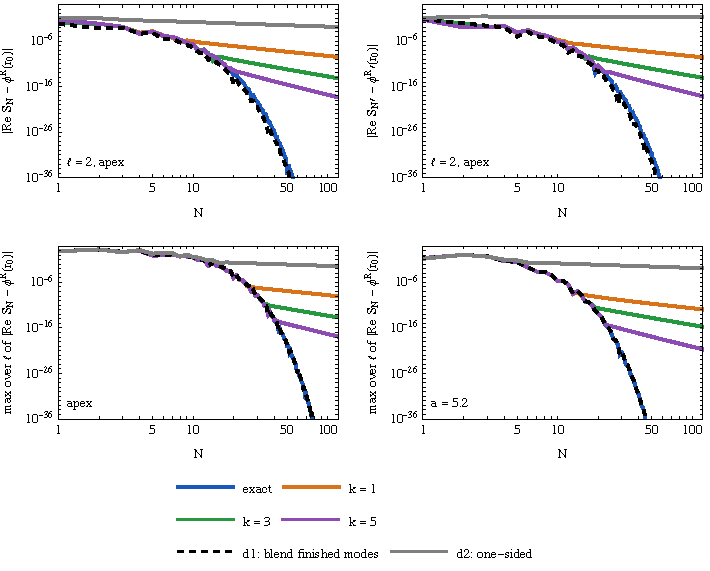
\includegraphics[width=0.85\textwidth]{fig_taylor_convergence.pdf}
\caption{Error of the Taylor partial sums at $r_0$ against the number of terms $N$. Top: $\ell=2$ about the apex, value (left) and radial derivative (right). Bottom: maximum over $\ell\le20$, about the apex (left) and $a_e=5.2$ (right). The controls d1 and d2 are described in Sec.~\ref{sec:controls}.}
\label{fig:taylor}
\end{figure}

\begin{table}[t]
\centering
\caption{Convergence of the Taylor sums at $r_0$: median fitted slopes of the real-part errors against $N$, and the maximum error over $\ell\le20$ at $N=120$ (apex).}
\label{tab:rates}
\small
\begin{tabular}{lcccll}
\toprule
 & \multicolumn{3}{c}{slope against $N$} & \multicolumn{2}{c}{max error, $N=120$}\\
case & value, apex & deriv., apex & deriv., $a_e=5.2$ & value & derivative\\
\midrule
exact & $0.199^N$ & geometric & $0.080^N$ & $<10^{-34}$ & $<10^{-32}$\\
$k=1$ & $-3.04$ & $-3.08$ & $-2.04$ & $8.7\times10^{-10}$ & $7.1\times10^{-10}$\\
$k=3$ & $-5.14$ & $-5.21$ & $-4.16$ & $1.8\times10^{-14}$ & $2.2\times10^{-14}$\\
$k=5$ & $-7.31$ & $-7.42$ & $-6.55$ & $1.1\times10^{-18}$ & $1.9\times10^{-18}$\\
\bottomrule
\end{tabular}
\end{table}

\subsection{Mode sums at the particle}
Summing the extracted modes, with the RR contribution taken from the real line, gives the residual at the particle (Table~\ref{tab:modesum}, Fig.~\ref{fig:modesum}).
In every case the error equals the error of the same sum built from the exact modes, so the Taylor step contributes nothing visible.
\begin{itemize}[leftmargin=*]
\item For the exact puncture, the $\ell$-truncation error comes from $h$ and falls as $(r_0/r_o)^\ell=3^{-\ell}$.
\item For the truncated punctures, it comes from the slowly convergent mode sum of $\rho^k$ at $\x_0$, as in any puncture scheme of that order.
\end{itemize}

\begin{table}[t]
\centering
\caption{Mode sums at $\x_0$ with $\ell_{\max}=20$. The errors equal those of the same sums built from exact modes.}
\label{tab:modesum}
\begin{tabular}{lllll}
\toprule
case & $\Phi_2^{\rm R}(\x_0)$ & error & $\partial_r\Phi_2^{\rm R}(\x_0)$ & error\\
\midrule
exact & $1.81388888879329$ & $9.6\times10^{-11}$ & $0.16061728353954$ & $4.1\times10^{-10}$\\
$k=1$ & $1.81198302958710$ & $1.9\times10^{-3}$ & $0.16042671314077$ & $1.9\times10^{-4}$\\
$k=3$ & $1.81390192019408$ & $1.3\times10^{-5}$ & $0.16062119295924$ & $3.9\times10^{-6}$\\
$k=5$ & $1.81388843917625$ & $4.5\times10^{-7}$ & $0.16061705873102$ & $2.3\times10^{-7}$\\
\midrule
exact value & $1.81388888888889$ & & $0.16061728395062$ & \\
\bottomrule
\end{tabular}
\end{table}

\begin{figure}[t]
\centering
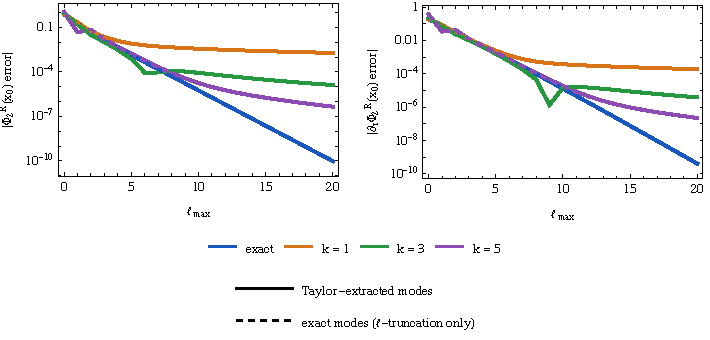
\includegraphics[width=0.85\textwidth]{fig_modesum.pdf}
\caption{Error of the mode sums for $\Phi_2^{\rm R}(\x_0)$ (left) and $\partial_r\Phi_2^{\rm R}(\x_0)$ (right) against $\ell_{\max}$. Solid: Taylor-extracted modes; dashed: exact modes. The two coincide.}
\label{fig:modesum}
\end{figure}

\subsection{Baseline: lower contours and \texorpdfstring{$\eta\to0$}{eta to 0}}
A simpler route is to use contours of decreasing apex height $\eta$, $y_\eta(a)=a+i\eta\big(1-4(a-r_0)^2\big)^6$, and read $\tilde\psi_\ell-\tilde\phi^{\rm P}_\ell$ at $r_0+i\eta$.
Figure~\ref{fig:eta} shows that the real part has a bias linear in $\eta$, with coefficient $-\Im\psiR{}'(r_0)$.
This is the shadow's derivative: $\Re\psiR(r_0+i\eta)=\Re\psiR(r_0)-\eta\,\Im\psiR{}'(r_0)+O(\eta^2)$.
At $\eta=1/128$ the bias is still $1.6\times10^{-3}$ for $\ell=2$.

Richardson extrapolation over the eight values $\eta=1,\dots,1/128$ recovers the exact case to $3\times10^{-15}$--$5\times10^{-11}$ for $\ell\le10$.
For truncated punctures it saturates at the $\eta^{k+2}\log\eta$ level ($10^{-10}$ for $k=1$).

We had expected this route to lose digits to cancellation between two singular quantities.
It does not: the field modes are only logarithmically singular at $r_0$, so $|\tilde\psi_\ell|$ and $|\tilde\phi^{\rm S}_\ell|$ at the apex stay of order one.
The cost is elsewhere: the source grows like $\eta^{-2}$ (to $1.3\times10^3$ at $\eta=1/128$), and resolving it needs more quadrature nodes (840 at $\eta=1$, 1120 at $\eta=1/128$).

\begin{figure}[t]
\centering
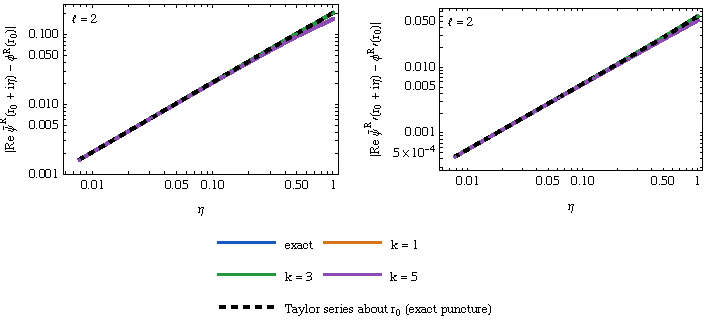
\includegraphics[width=0.85\textwidth]{fig_eta_baseline.pdf}
\caption{Baseline: bias of the residual read at $r_0+i\eta$ against $\eta$, $\ell=2$, value (left) and derivative (right). Dashed: the Taylor series about $r_0$ for the exact puncture.}
\label{fig:eta}
\end{figure}

\subsection{Controls: how the puncture is continued}\label{sec:controls}
Two alternative continuations of the puncture were tried.
\begin{itemize}[leftmargin=*]
\item \emph{d1: $H$-blend of the finished modes.}
The finished, differentiated SR puncture modes $P$ are kinked ($C^0$) at $r_0$.
Blending them directly, $P_{\rm in}+(P_{\rm out}-P_{\rm in})H$, gives the same real values as blending first and differentiating afterwards: the error is below $10^{-34}$.
We had predicted that this would fail, by analogy with the source (PRL Appendix~C, Step~6), where blending the finished source loses its $\delta$ terms.
The difference is that the puncture is a field.
For a kinked function, $\Lop\big[P_{\rm in}+(P_{\rm out}-P_{\rm in})H\big]$ contains $[P']\,\dext$ automatically, so the kink reproduces the $\delta$ in $\Lop P$.
The two continuations differ by a function that is imaginary on the axis and vanishes at $r_0$, a harmless shadow.
The finished SR source, by contrast, contains $\delta$ and $\delta'$ terms that no blend of functions can represent.
\item \emph{d2: one-sided continuation.}
Continuing $P_{\rm out}$ alone drops the kink, and hence the $\delta$ in $\Lop P$.
This fails, as it should.
Its real part is already wrong at $a_L$, by the jump times $\Theta(r_0-r)$.
The residual acquires a term $(i/\pi)c_\ell(z-r_0)\log(z-r_0)$, where $c_\ell$ is the dropped $\delta$ coefficient.
The value then converges only as $1/N$, and the derivative tends to the mean of the two one-sided derivatives, with error $|c_\ell|/2$ ($0.11$ for $\ell=0$, $0.24$ for $\ell=2$).
The mode sum for $\partial_r\Phi_2^{\rm R}(\x_0)$ is wrong by 13.
\end{itemize}
The requirement on the puncture is therefore the first consistency condition of the earlier note: the real part of the continued puncture on the axis must equal the modes of the 3D puncture on both sides of $r_0$.
Keeping the kink is enough; it does not matter whether the blend is applied before or after differentiation.

\section{Predictions and outcomes}
\begin{table}[h]
\centering
\begin{tabular}{p{0.44\textwidth}p{0.47\textwidth}}
\toprule
prediction & outcome\\
\midrule
Exact puncture: residual analytic at $r_0$; geometric convergence with ratio $\approx1/5$ from the apex. & Held: ratio $0.199$ against $0.196$; monodromy $<4\times10^{-20}$.\\
Truncated puncture: branch point at $r_0$; algebraic convergence $\sim N^{-k}$, worse for the derivative. & Algebraic held, but the exponent is $k+2$ for the value, because the mode functions are two orders smoother than the 3D field. The derivative is one order worse only off the vertical.\\
The puncture must be continued exactly as the source is, or the $\delta$ content is lost. & Did not hold: blending the finished, kinked puncture modes works. Dropping the kink fails.\\
Baseline loses about $2\log_{10}(1/\eta)$ digits to cancellation. & Did not hold: the field modes are only logarithmically singular. The limits are the $O(\eta)$ bias and the quadrature cost of the $\eta^{-2}$ source.\\
\bottomrule
\end{tabular}
\end{table}

\section{What this means beyond the toy}
\begin{itemize}[leftmargin=*]
\item \emph{The extraction works, and its accuracy is set by the puncture.}
With an exact puncture the Taylor step is essentially free.
With a truncated puncture it converges algebraically, at a rate set by the smoothness of the residual \emph{modes}, which is two orders better than that of the 3D residual.
In either case the final mode sum is limited by $\ell$-truncation, as in any puncture scheme.
\item \emph{What GR would need.}
The Taylor route needs $\psiR$ and $\psiR{}'$ at one contour point, and the residual source $\tilde s-\Lop\tilde\phi^{\rm P}_\ell$ on one small circle about that point, which lies wholly in the upper half-plane.
In GR the source there would come from the complex-$r$ angular quadrature of Appendix~C, which works at any point of the analytic region.
The Stage~14 lesson applies: one set of source evaluations per point can be shared across all modes.
\item \emph{Two routes, similar reach.}
The Taylor series and the $\eta$-extrapolation both reach $10^{-10}$ or better here.
The Taylor route is cleaner and works from a single contour.
The $\eta$ route needs no source derivatives, but needs several contours and more nodes near the axis.
For truncated punctures both are limited by the same branch point at $r_0$.
\item \emph{Precision and the shadow.}
The shadow of the residual is of order one and grows with $\ell$, to about $10$ at $\ell=20$.
In double precision this sets the absolute accuracy of the extracted modes.
That should be harmless for mode sums, whose terms are added absolutely, but it limits the relative accuracy of high-$\ell$ modes.
\item \emph{Limits of the test.}
\begin{itemize}
\item The toy is static, so it has no dissipative part. It tests the extraction of the local residual, which in GR carries the information that fluxes do not, such as the second-order redshift and binding energy.
\item The exact singular field is a finite closed form only because $\Phi^{\rm R}_1$ is linear.
\item The residual was made nonzero for every $\ell$ by injecting a harmonic field.
\item GR adds $m$-modes, two-dimensional angular integrals, window functions and $\ln\rho$ terms in the puncture, none of which is tested here.
\end{itemize}
\end{itemize}

\section{Reproducibility}
The test is \code{stage15\_residual\_extraction.wls}, in the folder\\ \code{Claude Implementation/Mathematica implementation/}.
It runs in 22 minutes (3 minutes with the \code{smoke} flag) and passes all 363 of its checks.
Results are in \code{results/stage15\_*.csv}, with a detailed summary in \code{results/stage15\_summary.md}.
The figures, each with a CSV, are in the folder \code{Claude Implementation/figures/residual/}.

\end{document}
